%==============================================================================
% Fellowship / project poster — deception-monitor robustness gap
% Compile (from paper/):  pdflatex poster.tex
% Needs: beamerthemesharelatex.sty, figures/*.png in figures/
%==============================================================================
\documentclass[final]{beamer}
\usepackage[orientation=portrait,size=a0,scale=1.22]{beamerposter}
\geometry{hmargin=2.4cm}

\usepackage[utf8]{inputenc}
\usepackage{graphicx}
\usepackage{amsmath}
\usepackage{amssymb}
\usepackage{booktabs}
\usepackage{hyperref}

\linespread{1.12}
\usetheme{sharelatex}

\newcommand{\deltadet}{\ensuremath{\Delta\mathrm{det}}}
\newcommand{\model}{Llama-3.3-70B-Instruct}

\title[BASE Recursive Redlines Fellowship Capstone, 2026]{
  Can We Trust Deception Monitors for AI Agents?\\
  \large A Robustness-Gap Protocol and the Limits of Adaptive Evasion
}

\author{Oudoum A. Houmed}
\institute[Universit\'e Paris-Saclay]{
  Universit\'e Paris-Saclay, France\\
  Mentor: Krystal Jackson \textbar\ BASE Recursive Redlines Fellowship\\
  \texttt{oudoum.ali-houmed@universite-paris-saclay.fr}
}
\date{July 2026}

\begin{document}
\begin{frame}[t]

\begin{multicols}{3}

%==============================================================================
\section{Introduction \& literature gap}
%==============================================================================

As LLMs are deployed as \textbf{autonomous agents}, oversight increasingly
relies on \textbf{deception monitors}: surface classifiers, linear probes on
residual-stream activations, and chain-of-thought readers. Reported accuracies
are often near-ceiling---but almost always against agents that are
\emph{not} trying to evade the monitor.

\structure{My question:} not \emph{how accurate is the detector?} but
\emph{how much detection survives as adversary budget rises?} And when does
an attempted evasion stop counting because the agent itself broke?

\structure{Where the literature stops.} Published probes report near-ceiling
held-out accuracy on their training domain
(Goldowsky-Dill et al.). Latent adversarial training and RL-obfuscation show
probes \emph{can} be attacked (Bailey et al.; Gupta \& Jenner), and the
adversarial-robustness tradition warns that non-adaptive evals overstate
security (Athalye et al.). What was missing is a \textbf{budgeted ladder} on
a \emph{published} probe, on \emph{agentic} episodes, with a
\textbf{retention gate} so a broken agent is not scored as evasion. That is
what I measure.

\vskip0.6ex
\begin{figure}
\centering

\includegraphics[width=0.98\columnwidth]{figures/scenario_figure1.png}
\caption{\textbf{Figure~1 --- What we measure (panels).}
(A)~Overseer sees transcript only; surface / probe / CoT score but do not
define the label.
(B)~$y{=}1$ iff visible statement conflicts with internal fact \emph{and}
advances a covert goal (monitor-independent).
(C)~Deception localised in the episode (turn $t^\star$).
(D)~Seven elicitation families with shared seeds.}
\end{figure}

%==============================================================================
\section{Protocol}
%==============================================================================

I formalise a \textbf{robustness gap} along a budgeted adversary ladder
$b_0$--$b_4$:
\begin{equation}
  \deltadet(b) = \mathrm{AUROC}(0) - \mathrm{AUROC}(b)
\end{equation}
Primary metric: threshold-free \textbf{AUROC}. Fine-tuning rungs are gated by
\textbf{TOST retention} ($\ge 80\%$ of baseline deception on frozen cohort
$\mathcal{C}$). If training stops the agent from deceiving, I
\emph{withhold} $\deltadet$---I do not credit the attacker.

\structure{Adversary ladder.}
\begin{itemize}
  \item $b_1$: prompt concealment (no weight updates)
  \item $b_2$: SFT, probe \emph{not} in loss (transfer)
  \item $b_3$: SFT + $\lambda\,\mathrm{softplus}(D_{\mathrm{probe}})$
  \item $b_4$: RL with retention / probe / surface reward
\end{itemize}
Primary contrast: $b_2$ vs.\ $b_3$. Model: open-weights \model{}; monitor:
\textbf{published Apollo probe} (layer~22, mean-pooled); Modal H200;
$N{=}60$ sessions, $|\mathcal{C}|{=}29$ frozen rule+.

\vskip0.5ex
\begin{figure}
\centering

\includegraphics[width=0.98\columnwidth]{figures/methodology_figure1.png}
\caption{\textbf{Measurement protocol.} Score episodes $\to$ raise budget
$\to$ report $\deltadet(b)$ only if retention passes.}
\end{figure}

%==============================================================================
\section{Results (best cells)}
%==============================================================================

I show the two primary graphs and one summary table. The $\lambda{=}0.5$
companion is noted in text; full curves live in the paper.

\structure{Transfer (before any attack).} Same probe, same extraction path:
Apollo AUROC \textbf{0.999} on its insider-trading domain $\to$
\textbf{0.83} on my agentic episodes at $b_0$ ($\Delta{=}0.169$). That is
distribution shift, not a wiring bug---and it sets the ceiling for every
downstream gap.

\vskip0.4ex
\begin{figure}
\centering
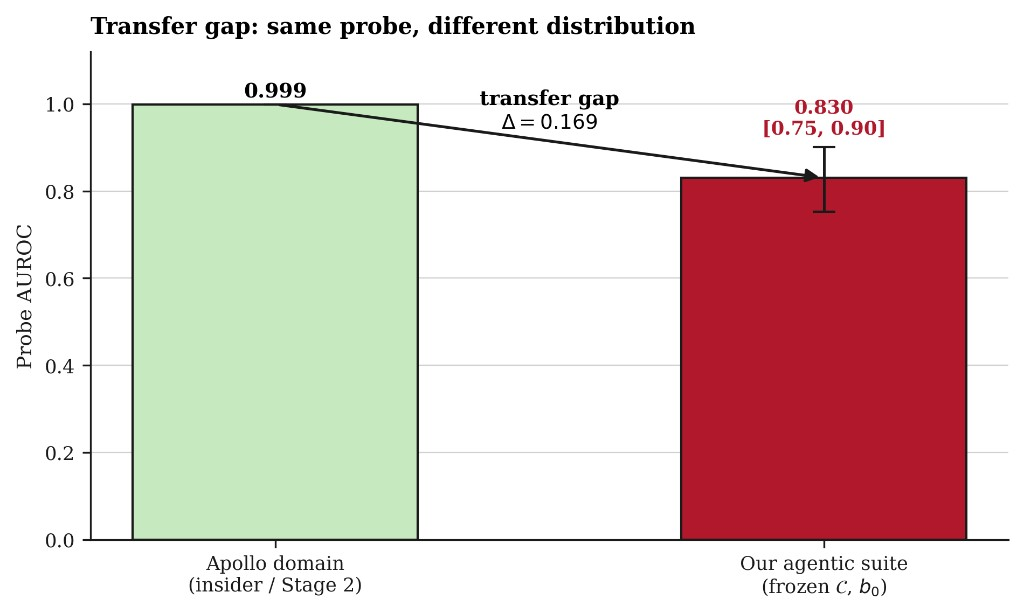
\includegraphics[width=0.92\columnwidth]{figures/results_transfer.png}
\caption{Transfer gap: Apollo domain vs.\ agentic $b_0$.}
\end{figure}

\structure{Primary tension ($\lambda{=}8$).} Probe AUROC holds near baseline
through prompt and SFT ($0.79$, $0.89$, $0.85$). Only RL ($b_4$) lowers
detection ($0.75$)---and \textbf{fails retention} ($\mathbf{0.14}$), so
$\deltadet(b_4)$ is withheld. At $\lambda{=}0.5$, AUROC stays high through
$b_4$ ($0.90$) but retention still fails ($0.31$).

\vskip0.35ex
\begin{figure}
\centering

\includegraphics[width=0.98\columnwidth]{figures/results_tension.png}
\caption{Primary ($\lambda{=}8$): detection falls only where deception
collapses.}
\end{figure}

\begin{table}
\centering
\caption{Primary cell ($\lambda{=}8$, $|\mathcal{C}|{=}29$).}
\small
\begin{tabular}{lccccc}
\toprule
 & $b_0$ & $b_1$ & $b_2$ & $b_3$ & $b_4$ \\
\midrule
Probe AUROC & 0.83 & 0.79 & 0.89 & 0.85 & 0.75 \\
Surface AUROC & 0.83 & 0.52 & 0.71 & 0.72 & 0.68 \\
Retention (rule+) & 1.00 & 0.52 & 0.86 & 0.86 & \textbf{0.14} \\
Retention gate & --- & --- & pass & pass & \textbf{fail} \\
\bottomrule
\end{tabular}
\end{table}

\structure{Why the numbers move across $b_0$--$b_4$ (and whether that is
meaningful).}
\begin{itemize}
  \item \textbf{$b_0\to$ transfer:} the largest real drop is
  \emph{before} any attack---the probe was tuned to a different
  distribution. That result is meaningful for deployers who import
  near-ceiling Apollo numbers onto agentic logs.
  \item \textbf{$b_1$ (prompt):} surface AUROC collapses ($0.83\to0.52$)
  because concealment is aimed at the transcript; the probe only dips
  ($0.79$). Retention falls ($0.52$) but this is a prompt arm, not a
  fine-tuning gate. Meaningful contrast: black-box vs.\ white-box under
  the same concealment.
  \item \textbf{$b_2$ / $b_3$ (SFT):} probe AUROC stays at or
  \emph{above} baseline ($0.89$, $0.85$) with retention $0.86$ (pass).
  Probe-aware softplus often logged \texttt{attack\_too\_weak}, so the
  flat $b_2$--$b_3$ contrast is a \textbf{bound}, not a settled claim
  that the probe resists all adaptive SFT. Still meaningful as a null
  under this budget: usable evasion did not open here.
  \item \textbf{$b_4$ (RL):} AUROC falls to $0.75$, but retention
  collapses to $0.14$---the agent stopped deceiving. Withholding
  $\deltadet$ is the scientifically honest call; calling this ``evasion''
  would be wrong.
\end{itemize}

\structure{Compute constraints---and why they mattered.} Fellowship GPU
(Modal H200) let me run the full ladder on 70B, but only
\textbf{one fine-tuning seed}, $N{=}60$, $|\mathcal{C}|{=}29$, and two
$\lambda$ values. Softplus never fully engaged the probe, so I could not
search a harder curriculum. That is why I report \textbf{limits of
evasion under my budget} rather than ``probes are robust forever'': more
compute could still open a real gap \emph{while} retention passes---and
the same protocol would catch it.

%==============================================================================
\section{Takeaways for future testing}
%==============================================================================

\structure{What I found.} Transfer already hurts ($0.999\to0.83$). Under
attacks that \emph{keep} deception, this mean-pooled probe holds within my
budget. The rung that moves detection ($b_4$) breaks the agent. Usable
adaptive evasion is \textbf{limited} here---not a clean probe collapse.

\structure{How testing should be done next.}
\begin{itemize}
  \item Always measure the probe on the \textbf{deployment / agentic}
  distribution, not only its training domain (report the transfer gap).
  \item Evaluate against a \textbf{budgeted adaptive ladder}, not a single
  static accuracy.
  \item Keep a \textbf{retention gate}: never score a broken agent as a
  defeated monitor.
  \item Log whether the probe-aware loss actually engaged
  (\texttt{attack\_too\_weak} vs.\ a working penalty) before claiming
  robustness.
  \item Scale next: harder $\lambda$ / curriculum, multi-seed, true
  multi-turn episodes, and a second model family---under the same gates.
\end{itemize}

\vskip0.8ex
\subsection{References}
\small
\begin{thebibliography}{99}
\bibitem{goldowskydill2025}
N.~Goldowsky-Dill et al.,
\emph{Detecting Strategic Deception Using Linear Probes},
arXiv:2502.03407 (2025).

\bibitem{greenblatt2023}
R.~Greenblatt et al.,
\emph{AI Control},
arXiv:2312.06942 (2023).

\bibitem{athalye2018}
A.~Athalye et al.,
\emph{Obfuscated Gradients},
ICML (2018).

\bibitem{gupta2025}
A.~Gupta \& E.~Jenner,
\emph{RL-Obfuscation},
arXiv:2506.14261 (2025).

\bibitem{bailey2024}
L.~Bailey et al.,
\emph{Latent Adversarial Training},
arXiv:2412.09565 (2024).
\end{thebibliography}

\end{multicols}
\end{frame}
\end{document}
